\documentclass[twocolumn, 10pt,a4j]{jsarticle}
  \usepackage{here}
  \usepackage{amsmath}
  \usepackage[dvipdfmx]{graphicx}
  \usepackage{url}
  % プリアンブル
  \title{\vspace{-2.5cm}振動の計測と制御}
  \author{1610581 堀田 大地}
  \date{2018/7/26}
  \begin{document}
  \maketitle{}
  \section{結果}
    結果画像を図11,12,13に示した.図3より,60Hzが共振周波数である.

    \begin{figure}[H]
      % 図6
      \begin{center}
        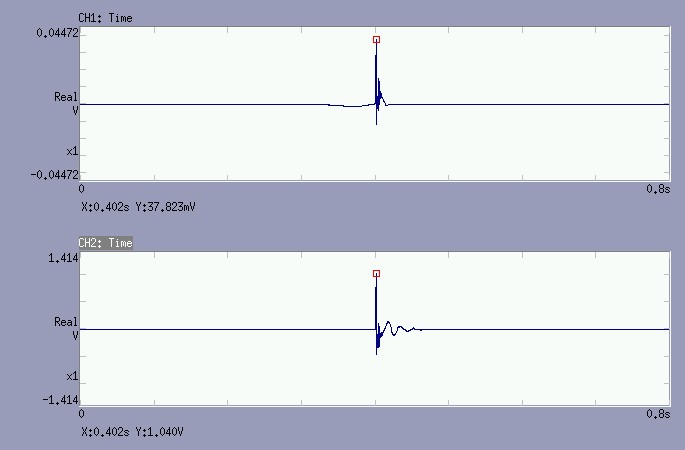
\includegraphics[width=7cm]{../img/experiments/011.png}
        \caption{インパクトハンマーの信号と振動系の加速度センサー信号の時間軸波形}
      \end{center}
    \end{figure}
    \begin{figure}[H]
      % 図6
      \begin{center}
        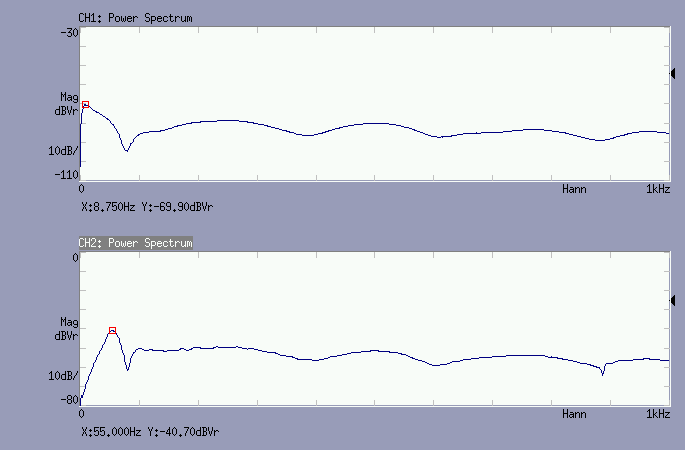
\includegraphics[width=7cm]{../img/experiments/013.png}
        \caption{インパクトハンマーから得られた信号$G_{x}$のパワースペクトルと1自由度振動系に取りつけた加速度センサからの信号$G_{y}$のパワースペクトル}
      \end{center}
    \end{figure}
    \begin{figure}[H]
      % 図6
      \begin{center}
        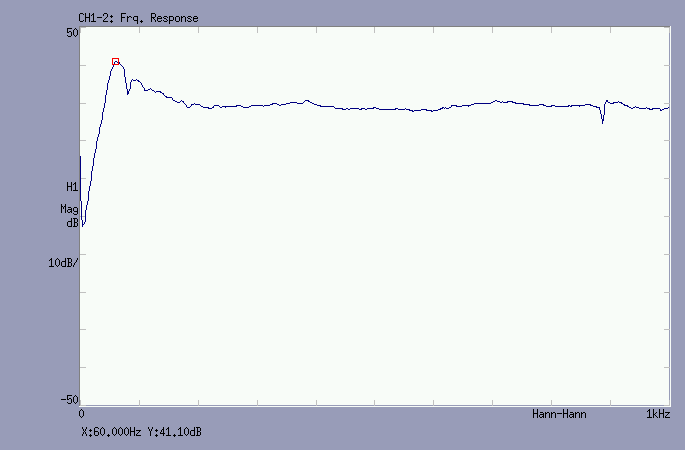
\includegraphics[width=7cm]{../img/experiments/015.png}
        \caption{伝達関数$H = G_{y}/G_{x}$の周波数応答スペクトル (周波数領域における入出力比)}
      \end{center}
    \end{figure}
  \end{document}